\documentclass[a4paper,11pt]{article}

\newcommand{\authorinfo}{Paul Bienkowski, Konstantin Kobs}
\newcommand{\titleinfo}{Robotics Assignment \#05}

% PREAMBLE ===============================================================

\usepackage[german,ngerman]{babel}
\usepackage[utf8]{inputenc}
\usepackage[T1]{fontenc}
\usepackage[top=1.3in, bottom=1in, left=1.0in, right=0.6in]{geometry}
\usepackage{lmodern}
\usepackage{amssymb}
\usepackage{mathtools}
\usepackage{amsmath}
\usepackage{enumerate}
\usepackage{pgfplots}
\usepackage{breqn}
\usepackage{tikz}
\usepackage{fancyhdr}
\usepackage{multicol}
\usepackage{gensymb}
\usepackage{listings}
\lstset{tabsize=2}

\allowdisplaybreaks

\usetikzlibrary{calc}
\usetikzlibrary{patterns}

\author{\authorinfo}
\title{\titleinfo}
\date{\today}

\pagestyle{fancy}
\fancyhf{}
\fancyhead[L]{\authorinfo}
\fancyhead[R]{\titleinfo}
\fancyfoot[C]{\thepage}

\begin{document}
\maketitle
\begin {enumerate}
	\item[\textbf{Task 5.1.}]
		We wrote a script in python to calculate the basis splines. These are the plots we got from our code:
		
		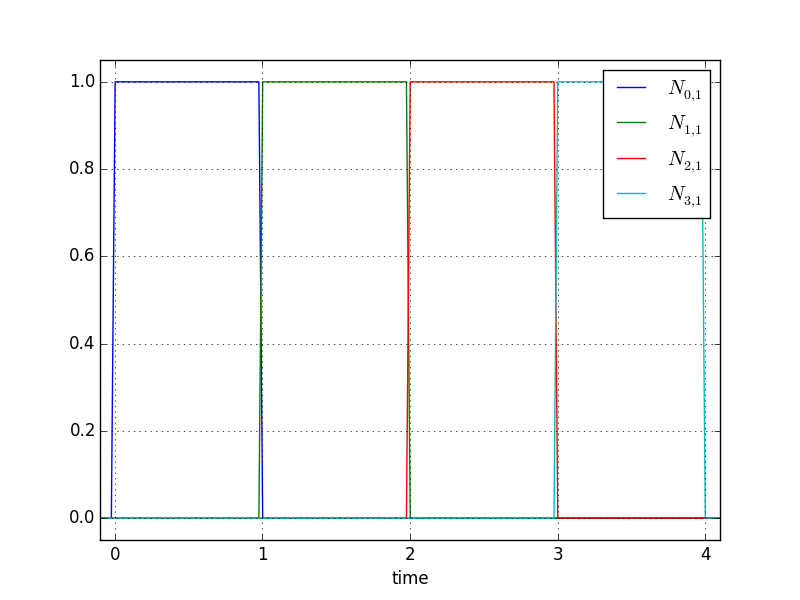
\includegraphics[width=0.5\textwidth]{5-1-k=1}
		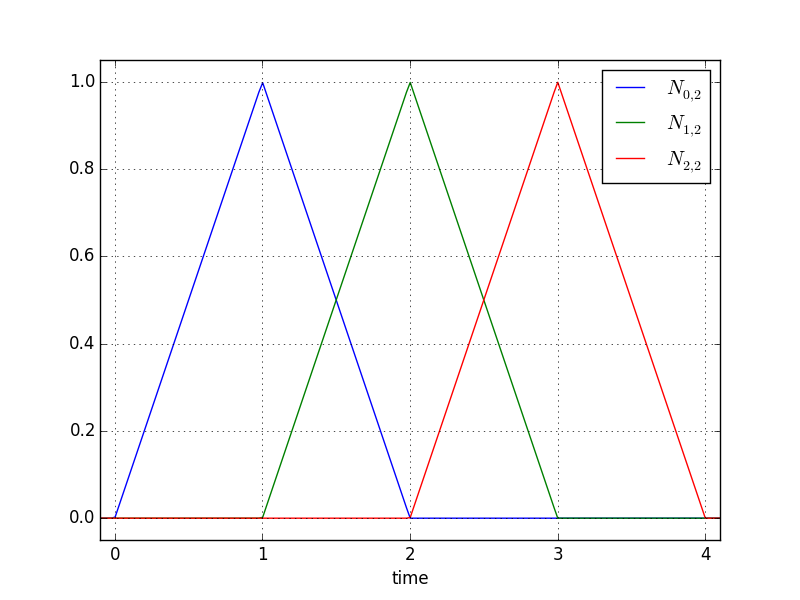
\includegraphics[width=0.5\textwidth]{5-1-k=2}
		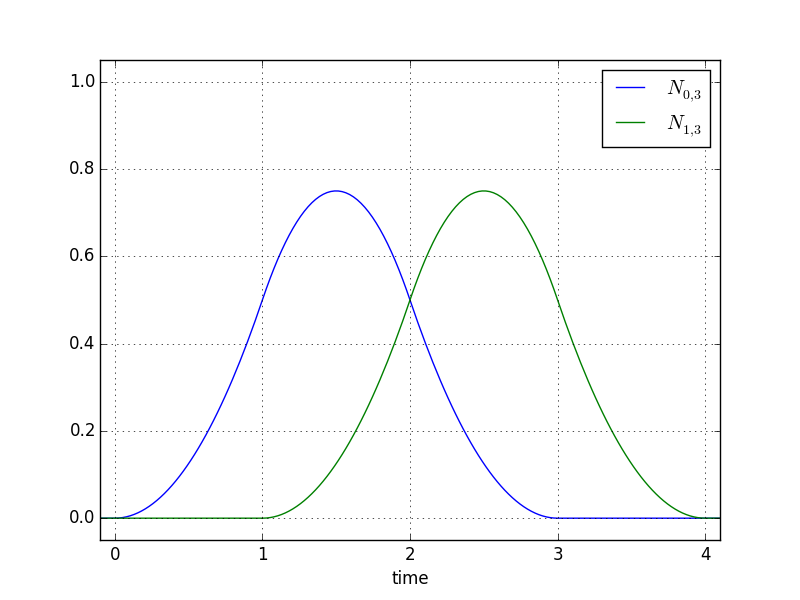
\includegraphics[width=0.5\textwidth]{5-1-k=3}
		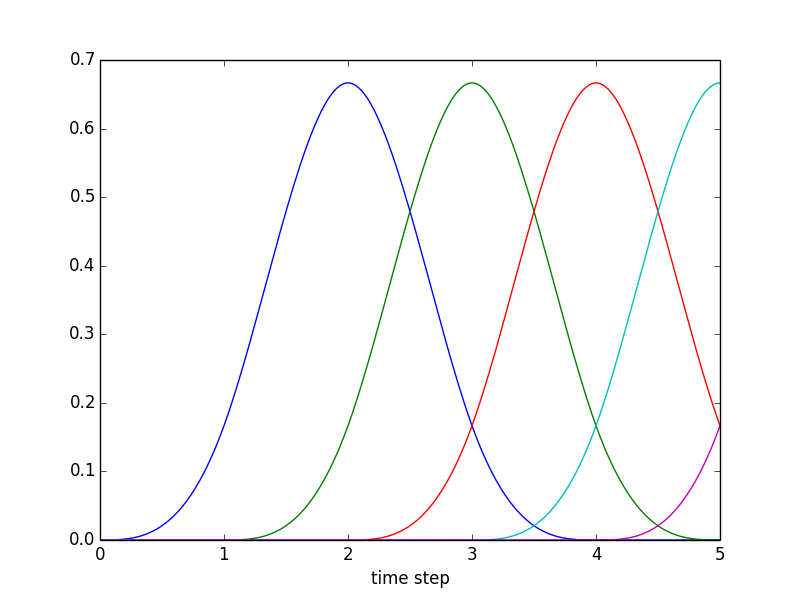
\includegraphics[width=0.5\textwidth]{5-1-k=4}
		
		The code is the following and can be found in 5.1.py:
		
		\lstinputlisting[language=python, frame=single, breaklines=true]{5.1.py}
		
	\item[\textbf{Task 5.2.}]
		
	\item[\textbf{Task 5.3.}]
		
	\item[\textbf{Task 5.4.}]
		
		
		
\end {enumerate}
\end{document}
